\documentclass[unicode,11pt,a4paper,oneside,numbers=endperiod,openany]{scrartcl}
\usepackage{amsmath} % for \text command
\usepackage{ifthen}
\usepackage[utf8]{inputenc}
\usepackage{graphics}
\usepackage{graphicx}
\usepackage{hyperref}

\pagestyle{plain}
\voffset -5mm
\oddsidemargin  0mm
\evensidemargin -11mm
\marginparwidth 2cm
\marginparsep 0pt
\topmargin 0mm
\headheight 0pt
\headsep 0pt
\topskip 0pt        
\textheight 255mm
\textwidth 165mm

\newcommand{\duedate} {}
\newcommand{\setduedate}[1]{%
\renewcommand\duedate {Due date:~ #1}}
\newcommand\isassignment {false}
\newcommand{\setassignment}{\renewcommand\isassignment {true}}
\newcommand{\ifassignment}[1]{\ifthenelse{\boolean{\isassignment}}{#1}{}}
\newcommand{\ifnotassignment}[1]{\ifthenelse{\boolean{\isassignment}}{}{#1}}

\newcommand{\assignmentpolicy}{
\begin{table}[h]
\begin{center}
\scalebox{0.8} {%
\begin{tabular}{|p{0.02cm}p{16cm}|}
\hline
&\\
\multicolumn{2}{|c|}{\Large\textbf{HPC Lab for CSE 2024 ---  Submission Instructions}}\\
\multicolumn{2}{|c|}{\large\textbf{(Please, notice that following instructions are mandatory: }}\\
\multicolumn{2}{|c|}{\large\textbf{submissions that don't comply with, won't be considered)}}\\
&\\
\textbullet & Assignments must be submitted to \href{https://moodle-app2.let.ethz.ch/course/view.php?id=22516}{Moodle} (i.e. in electronic format).\\
\textbullet & Provide both executable package and sources (e.g. C/C++ files, Matlab). 
If you are using libraries, please add them in the file. Sources must be organized in directories called:\\
\multicolumn{2}{|c|}{\textit{Project\_number\_lastname\_firstname}}\\
& and  the  file must be called:\\
\multicolumn{2}{|c|}{\textit{project\_number\_lastname\_firstname.zip}}\\
\multicolumn{2}{|c|}{\textit{project\_number\_lastname\_firstname.pdf}}\\
\textbullet &  The TAs will grade your project by reviewing your project write-up, and looking at the implementation 
                 you attempted, and benchmarking your code's performance.\\

\textbullet & You are allowed to discuss all questions with anyone you like; however: (i) your submission must list anyone you discussed problems with and (ii) you must write up your submission independently.\\
\hline
\end{tabular}
}
\end{center}
\end{table}
}
\newcommand{\punkte}[1]{\hspace{1ex}\emph{\mdseries\hfill(#1~\ifcase#1{Points}\or{Points}\else{Points}\fi)}}


\newcommand\serieheader[6]{
\thispagestyle{empty}%
\begin{flushleft}

\includegraphics[width=0.4\textwidth]{ETHlogo_13}
\end{flushleft}
  \noindent%
  {\large\ignorespaces{\textbf{#1}}\hspace{\fill}\ignorespaces{ \textbf{#2}}}\\ \\%
  {\large\ignorespaces #3 \hspace{\fill}\ignorespaces #4}\\
  \noindent%
  \bigskip
  \hrule\par\bigskip\noindent%
  \bigskip {\ignorespaces {\Large{\textbf{#5}}}
  \hspace{\fill}\ignorespaces \large \ifthenelse{\boolean{\isassignment}}{\duedate}{#6}}
  \hrule\par\bigskip\noindent%  \linebreak
 }

\makeatletter
\def\enumerateMod{\ifnum \@enumdepth >3 \@toodeep\else
      \advance\@enumdepth \@ne
      \edef\@enumctr{enum\romannumeral\the\@enumdepth}\list
      {\csname label\@enumctr\endcsname}{\usecounter
        {\@enumctr}%%%? the following differs from "enumerate"
	\topsep0pt%
	\partopsep0pt%
	\itemsep0pt%
	\def\makelabel##1{\hss\llap{##1}}}\fi}
\let\endenumerateMod =\endlist
\makeatother




\usepackage{textcomp}






\begin{document}


\setassignment
\setduedate{Friday 12 April 2024, 23:59 (midnight)}

\serieheader{AI in the Sciences and Engineering}{2024}
            {Student: Carla Judith L\'opez Zurita}
            {}{Project 1}{}
\newline

The main objective of the project is to apply the concepts learned in class by
implementing our own machine learning algorithms. The tasks
are related to solving differential equations using a Physics Informed Neural
Network (PINN), as well as solving an inverse problem. The project also includes 
a regression problem and an optional task to test the robustness of a given PINN.
My attempt at solving each of the mentioned tasks will be described in detail below.



\section{Task 1:  PINNs for solving PDEs}
The first task consists in solving the system of equations given by the heat
equation for a fluid and a solid in a thermal storage. The equations are as follows:
\begin{equation}
    \frac{\partial T_f}{\partial t} + U_f \frac{\partial T_f}{\partial x} = \alpha_f \frac{\partial^2 T_f}{\partial x^2} - h_f(T_f - T_s) \quad \text{for} \quad x \in [0, 1], \quad t \in [0, 1],
\end{equation}
\begin{equation}
     \frac{\partial T_s}{\partial t} = \alpha_s \frac{\partial^2 T_s}{\partial x^2} + h_s(T_f - T_s) \quad \text{for} \quad x \in [0, 1], \quad t \in [0, 1],
\end{equation}
with appropriate boundary conditions and constant values defined in the project description.
To solve this problem, a two-outputs neural network $(t,x) \to
(T^{\theta}_f,T^{\theta}_s)$, with tunable parameters $\theta$, was trained.
The implementation was based on the Tutorial 2 presented in class. It consists on a
very straight-forward implementation of a feed-forward neural network using
pytorch. 
The neural network uses SiLU and Linear activation functions and has with adjustable
number of layers and neurons, for which I chose 2 and 100 respectively. The numbers
reveal a dense but not very deep network.
The neural network was trained using the LBFGS optimizer with ten thousand
iterations done over a single epoch. The optimizer parameters include a learning rate 
of 0.5, a history size of 150, with a strong Wolfe condition. The loss
function is a custom function that consists of the sum of the mean squared
error for the PDEs and the boundary conditions. 
Both Dirichlet and Von Neumann boundary conditions were used, with the latter
requiring a derivative. This and all other derivatives required by the system of
equations were calculated using the autograd function.
The results of the loss function when training are shown in Figure
\ref{fig:task1_loss}. The plot shows the loss function decreasing steadily and
smoothly, reaching a minimum value of $1\times 10^{-04}$.
\begin{figure}[h]
    \centering
    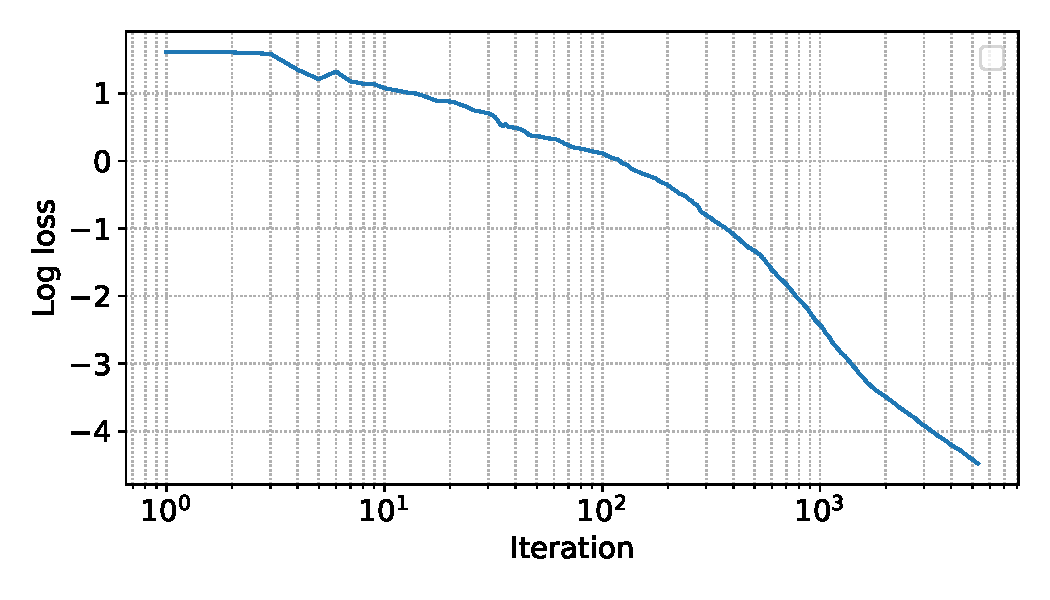
\includegraphics[width=0.6\textwidth]{../Proj1_Y24/Task1/loss.pdf}
    \caption{Loss function during training.}
    \label{fig:task1_loss}
\end{figure}
Figure \ref{fig:task1} shows the visualization of the results of the PINN for
the heat equation. The plot shows the approximate solution for the fluid $T_f$
and solid phases $T_s$ at the end of the simulation. The results show a smooth
and continuous solution that seems to be a good approximation of the real system.
\begin{figure}[h]
    \centering
    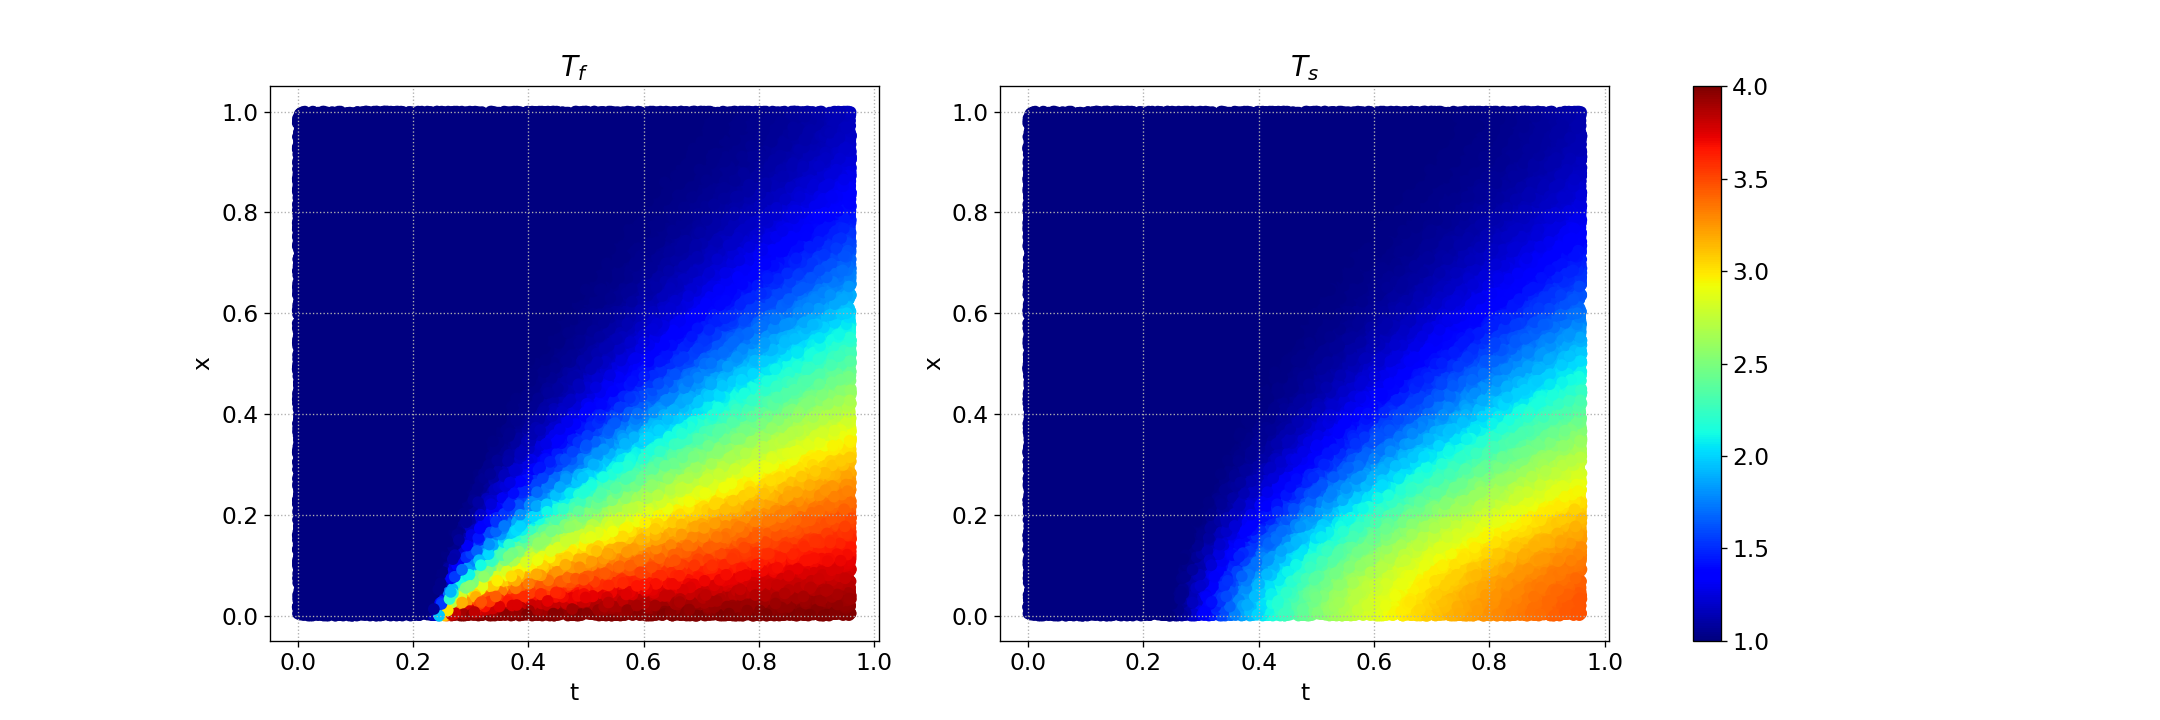
\includegraphics[width=1.2\textwidth]{../Proj1_Y24/Task1/output.png}
    \caption{Approximate solution for the fluid $T_f$ and solid temperatures $T_s$.}
    \label{fig:task1}
\end{figure}


\section{Task 2: PDE-Constrained Inverse Problem}
In the second task, the goal is to solve an inverse problem for the heat
equation
\begin{equation}
    \frac{\partial T_f}{\partial t}(x,t) + U_f(t)\frac{\partial T_f}{\partial x}(x,t) = \alpha \frac{\partial^2 T_f}{\partial x^2} (x,t) - h_f(T_f(x,t)-T_s(x,t)) \quad \text{for} \quad x \in [0, 1], \quad t \in [0, 8],
\end{equation}
with Dirichlet boundary conditions and initial condition. The inverse problem
consists in finding the value of the solid temperature $T_s$ through all 8
phases of the simulation. The problem is solved by training two different neural
network with the same architecture, each one with a different output
corresponding to the fluid and solid temperatures. The neural network follows a
similar architecture as the one in Task 1, but has a Tanh activation function
instead and uses Xavier initialization. 
The neural network is trained using the
LBFGS optimizer with 10000 iterations and two epochs, with a learning rate of 0.3. The loss
function is again a custom function that depends on the output of both neural
networks, the PDEs and the boundary conditions. The plot regarding the loss
function during training is shown in Figure \ref{fig:task2_loss}. The plot shows
the loss function decreasing steadily and smoothly, but does not reach such a
low minimum value as in Task 1, reaching instead a minimum value of $-0.827$.
When training for longer periods, the loss function didn't decrease further.
\begin{figure}
    \centering
    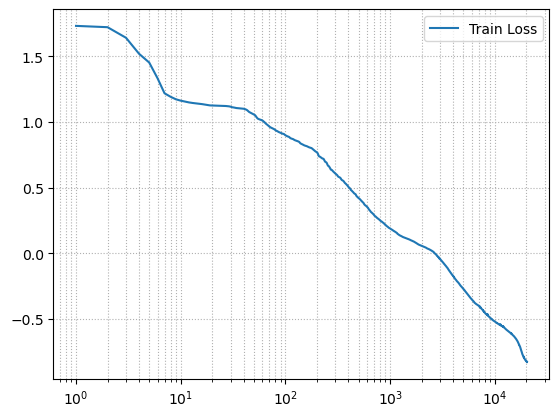
\includegraphics[width=0.6\textwidth]{../Proj1_Y24/Task2/loss.png}
    \caption{Loss function during training.}
    \label{fig:task2_loss}
\end{figure}
The results of the inverse problem are shown in Figure \ref{fig:task2}. The plot
show a good approximation of the solid temperature $T_s$ through all 8 phases of
the simulation.
\begin{figure}[h]
    \centering
    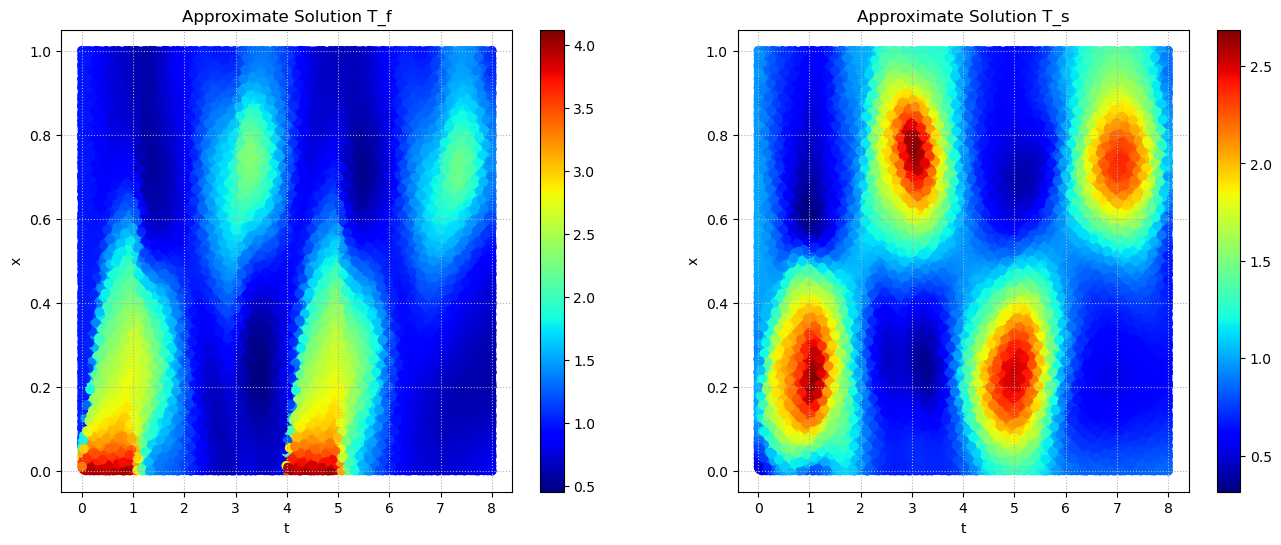
\includegraphics[width=\textwidth]{../Proj1_Y24/Task2/output.png}
    \caption{Results of the inverse problem for the system of equations, showing the fluid  $T_f$ and solid temperature $T_s$.}
    \label{fig:task2}
\end{figure}
We can see the ``discovered'' physics in the plot, as the solid temperature
$T_s$
shows an interesting pattern that seems to be related to the fluid temperature
$T_f$.

\section{Task 3: Applied Regression}
This task consists in solving a regression problem using a neural network. The
problem is based on the California Housing dataset \cite{wang_california_housing_1990}, and based on the Tutorial
``California Housing analysis and preciction'' by Larchenko \cite{Larchenko2019}
. The goal is to predict the
median house value for California districts, given a set of features. I used the
ones present on the dataset and derived by Larchenko. The
dataset is divided into training and testing sets, with 80\% of the data used
for training and the remaining 20\% for testing. The neural network used for
this task has a single output and uses the ReLU activation function. The network
has two hidden layers with 100 neurons each. The network is trained using the
Adam optimizer with a learning rate of 0.001 and a batch size of 32. The loss
function used is the mean squared error. 
The results of the loss function during training are shown in Figure \ref{fig:task3_loss}.
\begin{figure}[h]
    \centering
    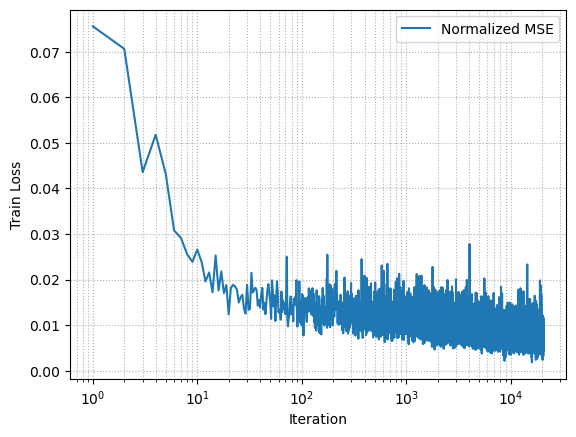
\includegraphics[width=0.6\textwidth]{../Proj1_Y24/Task3/loss.png}
    \caption{Loss function during training.}
    \label{fig:task3_loss}
\end{figure}
% \section{Task 4: Robustness of PINNs and Transferability (Optional)}


\bibliographystyle{plain}
\bibliography{bibliography}

\end{document}
